\subsection{3 Sites Results}

Let's first take a look at the impact of diversions with 60min
lead time. Figure \ref{fig:3sites_extreme} shows how extreme
waiting cases are reduced. First thing to notice is that
different sites start out differently. This is caused by
different number of machines they have. York Ave has 4 machines,
so it already enjoys a lot of pooling effect. That's why patients
generally wait less there. However, as we can see in Figure \ref{fig:3sites_extreme},
diversions reduce extreme waiting cases for all sites, most
prominently at sites with fewer machines.

Since we're optimizing $l2$-norm of waiting time vector.
It's understandable that we can reduce extreme waiting time,
potentially by propping up waiting time for other patients.
So it's interesting to look at how we're doing on mean waiting
time.

\begin{figure}[htp]
\centering
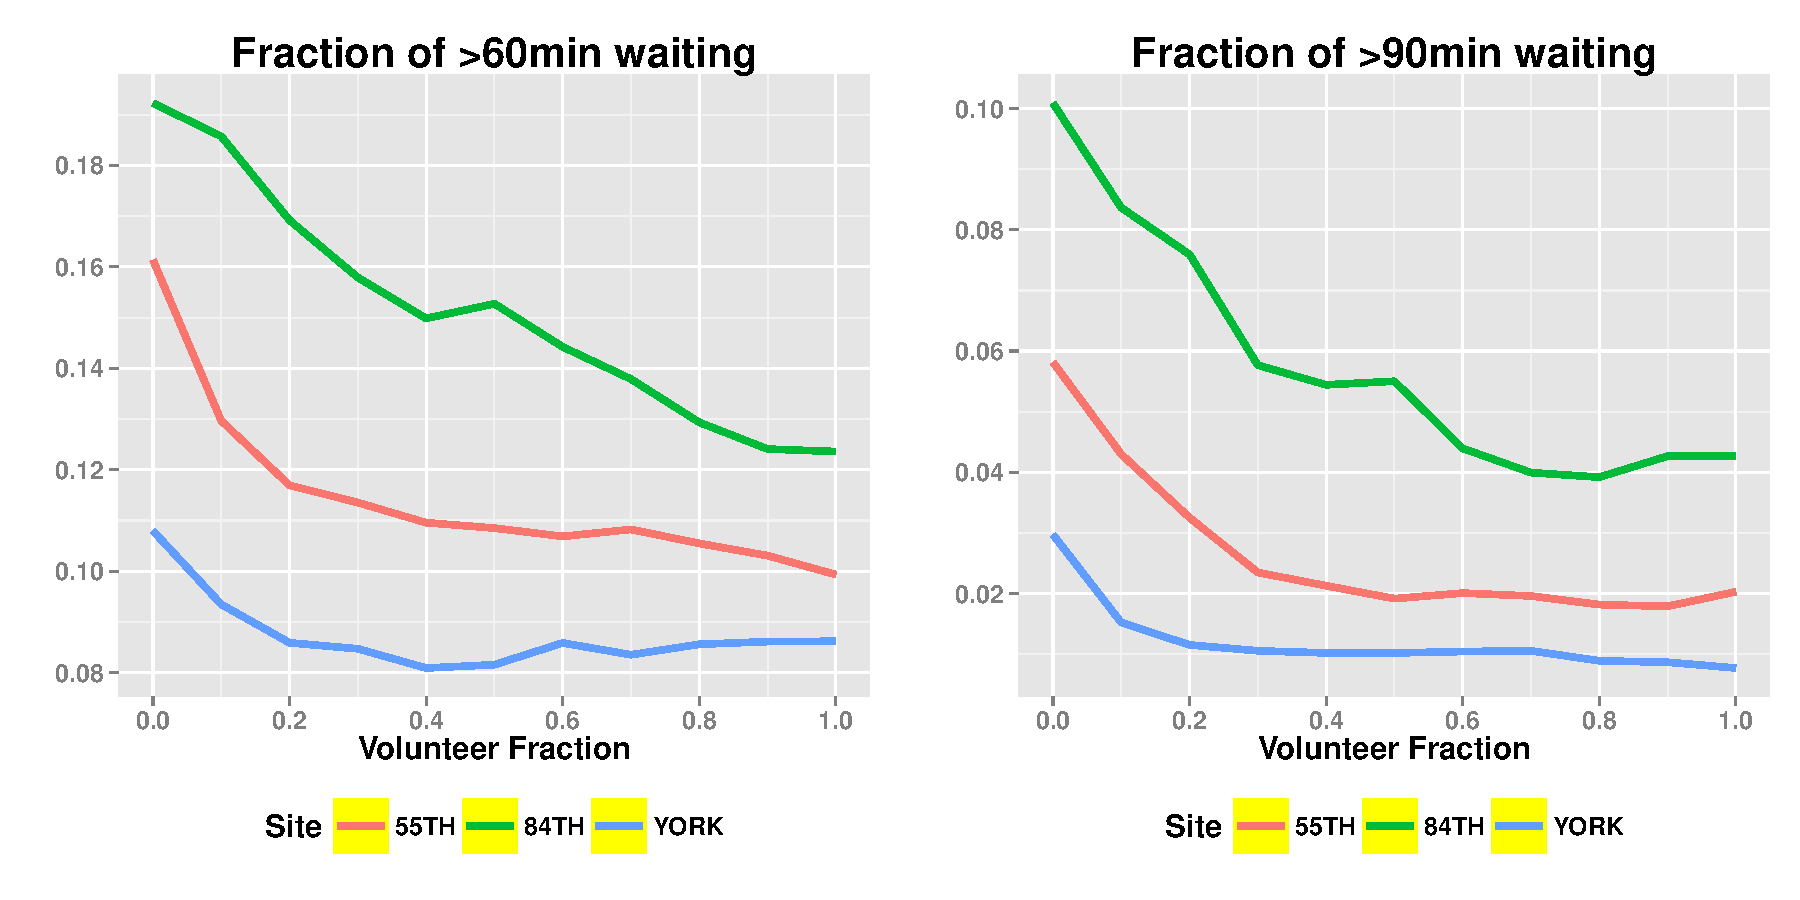
\includegraphics[width=.95\textwidth]{chap3/numeric/pic/3sites_extreme}
\caption{The impact on extreme waiting by diversions.}
\label{fig:3sites_extreme}
\end{figure}

Figure \ref{fig:3sites_wait_over} shows that we actually
reduced mean waiting time for all sites and the reduction
for 84th St and 55th St is again quite significant.
Not only that, we also reduced mean overtime for all sites, so
the staff can go home earlier. This means that we can finish
the same amount of work within shorter amount of working time.

\begin{figure}[htp]
\centering
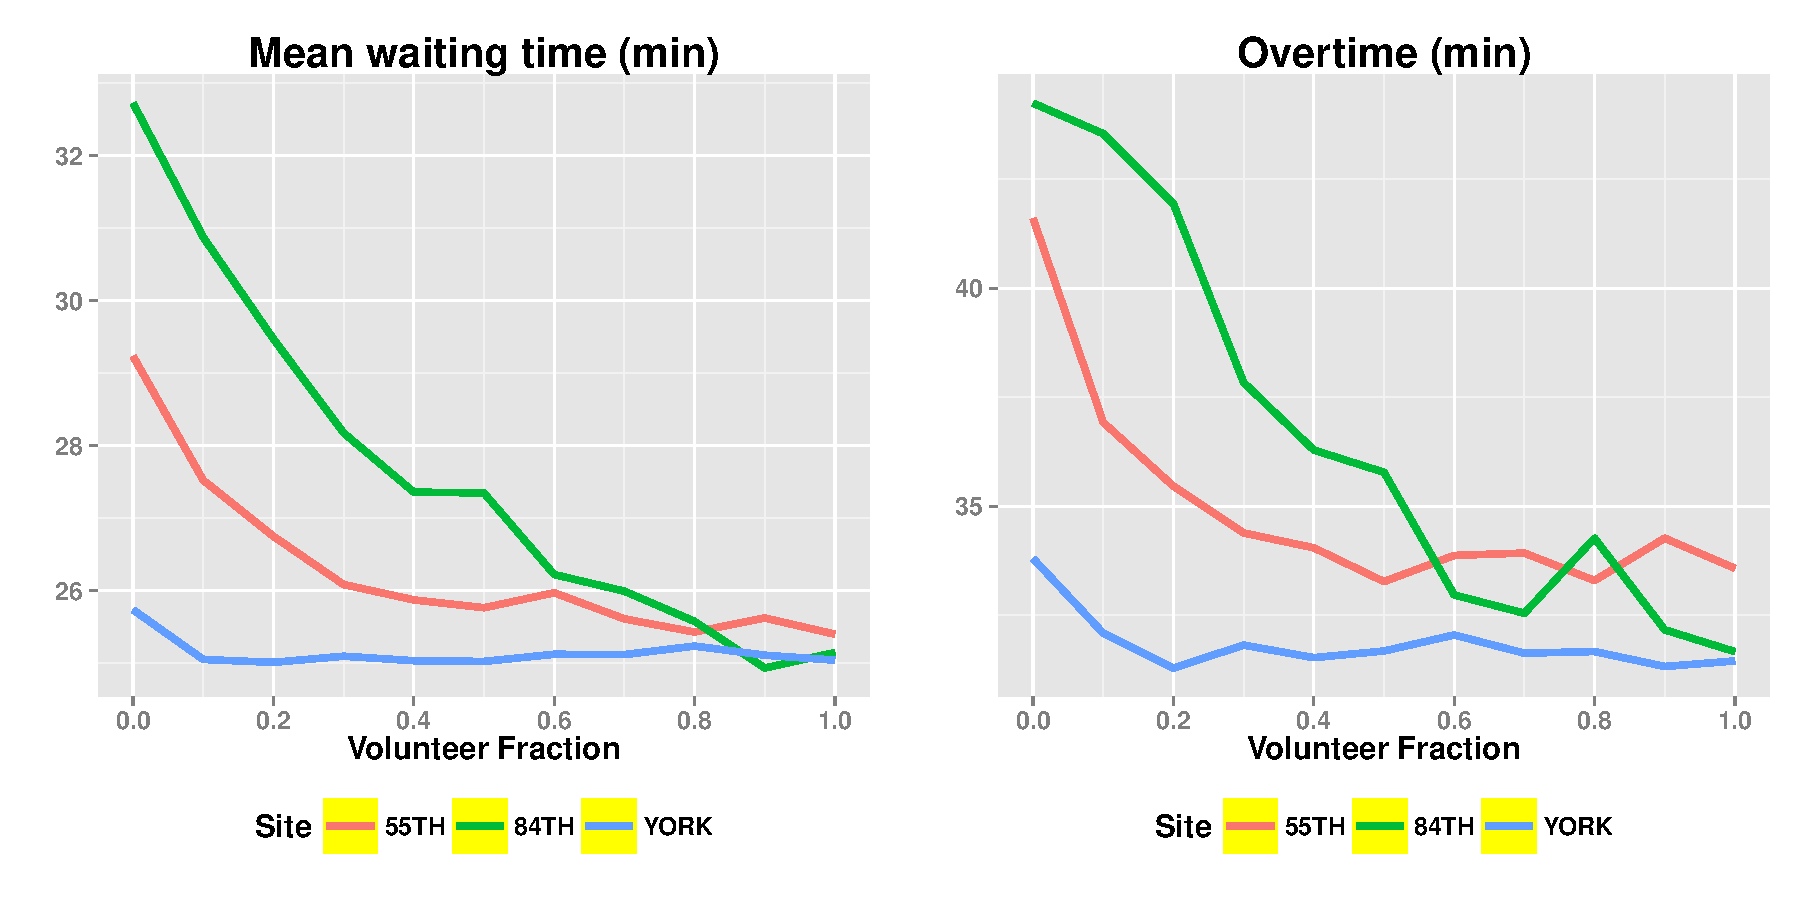
\includegraphics[width=.95\textwidth]{chap3/numeric/pic/3sites_wait_over}
\caption{The impact on mean waiting times and mean site overtimes by diversions.}
\label{fig:3sites_wait_over}
\end{figure}

The explanation comes from Figure \ref{fig:3sites_idle}. By
diverting patients to non-congested site, we actually reduce
idle time there. Because we have make use of some machine time that
would be otherwise wasted in idling, we can finish more work
in same amount of time, resulting in less backlog and congestion.

\begin{figure}[htp]
\centering
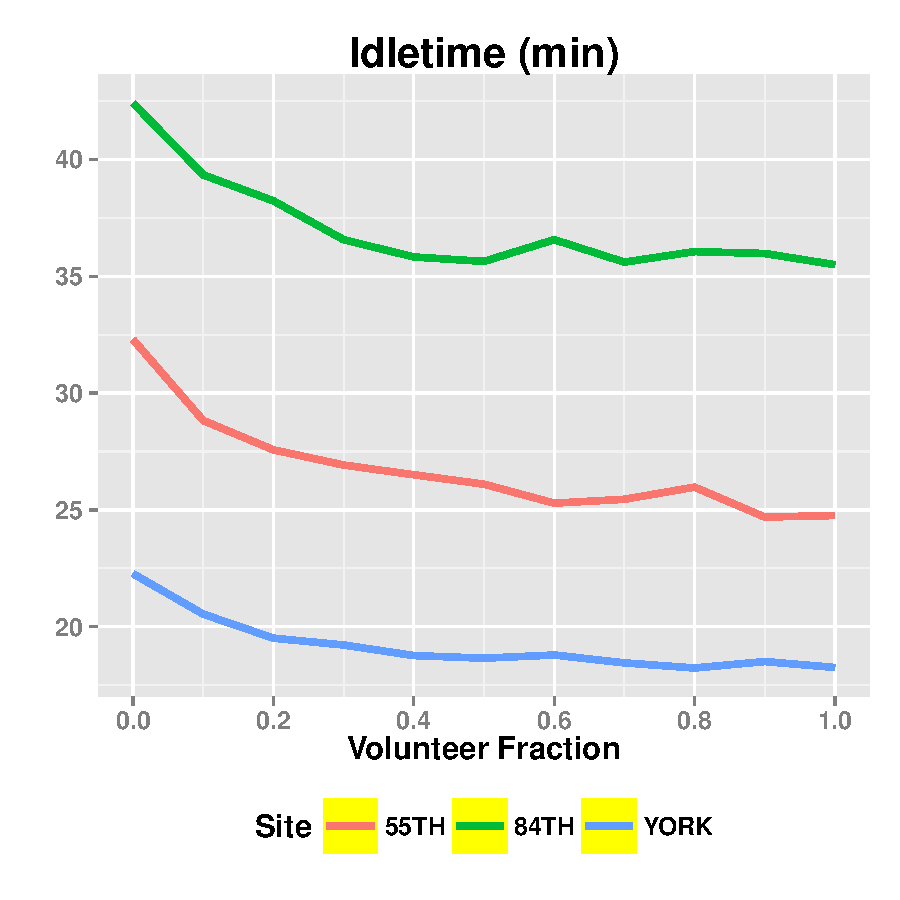
\includegraphics[width=.6\textwidth]{chap3/numeric/pic/3sites_idle}
\caption{The impact on mean idle times.}
\label{fig:3sites_idle}
\end{figure}

Figure \ref{fig:3sites_gain_flow} shows that the most diversions are
into York Ave and patients who are diverted to York Ave enjoys the
most reduction in waiting time. This is quite intuitive that
the pooling effect at York Ave gives it more processing capability.
So it has more slack to take in more patients than the other two
sites can. No matter which site the patient is diverted to,
he/she always enjoys significant reduction in waiting time, this
should serve as great incentive for them to cooperate if they
have the flexbility to.

\begin{figure}[htp]
\centering
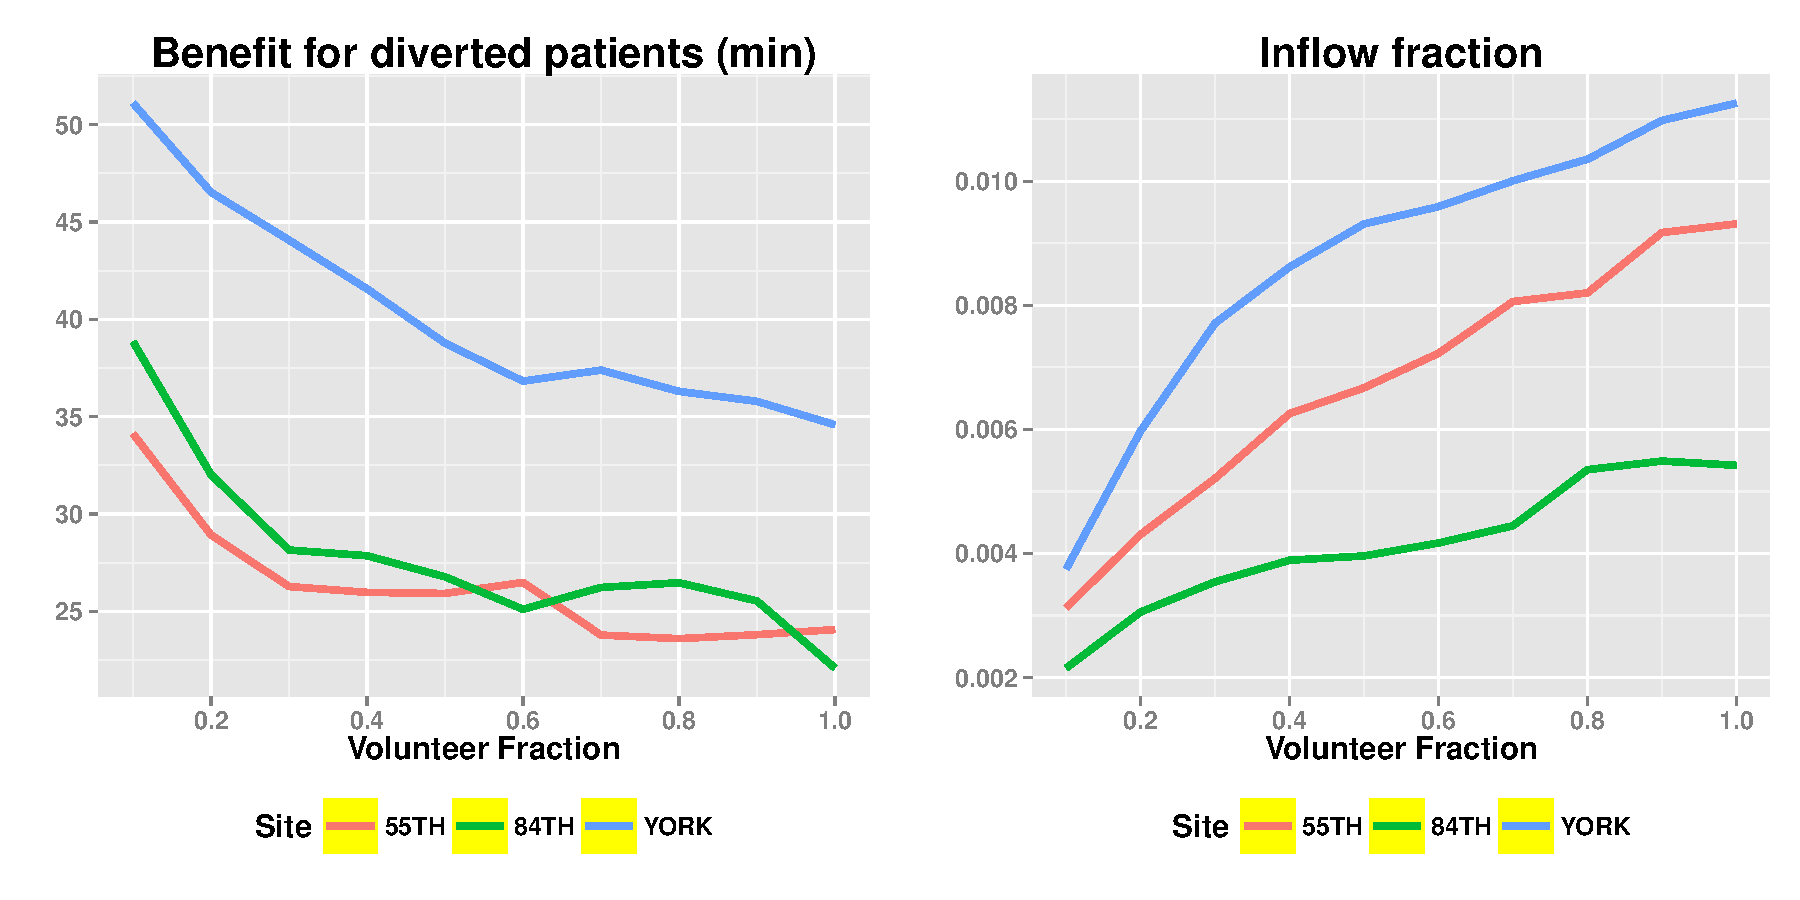
\includegraphics[width=.95\textwidth]{chap3/numeric/pic/3sites_gain_flow}
\caption{The amount of diversion into each site and reduction of waiting time
enjoyed being diverted into each site.}
\label{fig:3sites_gain_flow}
\end{figure}

Overall, we can see across all the figures, that the system performance
improves fastest when we only have very little fraction of patients as
volunteers. In other words, diversions can rapidly improve system
performance with very little flexbility. This is desirable since
benefits seen in limited trial can give practioner more confidence
to implement this in more full scope.

Figure \ref{fig:3sites_all} shows the overall system performance for both 60min lead time
and 90min lead time case. It reiterates the discussion above. Overall,
with 60min lead time and 40\% volunteers, we bring down the fraction
of over 60min cases from 13.5\% to 9.7\%, and the fraction of
over 90min cases from 4.7\% to 1.8\%. Both overtime and idle time
are significantly improved.

However, we would like to stress that even with 90min lead time, the diversions
still bring much improvement, not too much different from
the performance with 60min lead time. This has quite important practical
implication since longer lead time makes it easier for patients to be
diverted to different sites.

\begin{figure}[htp]
\centering
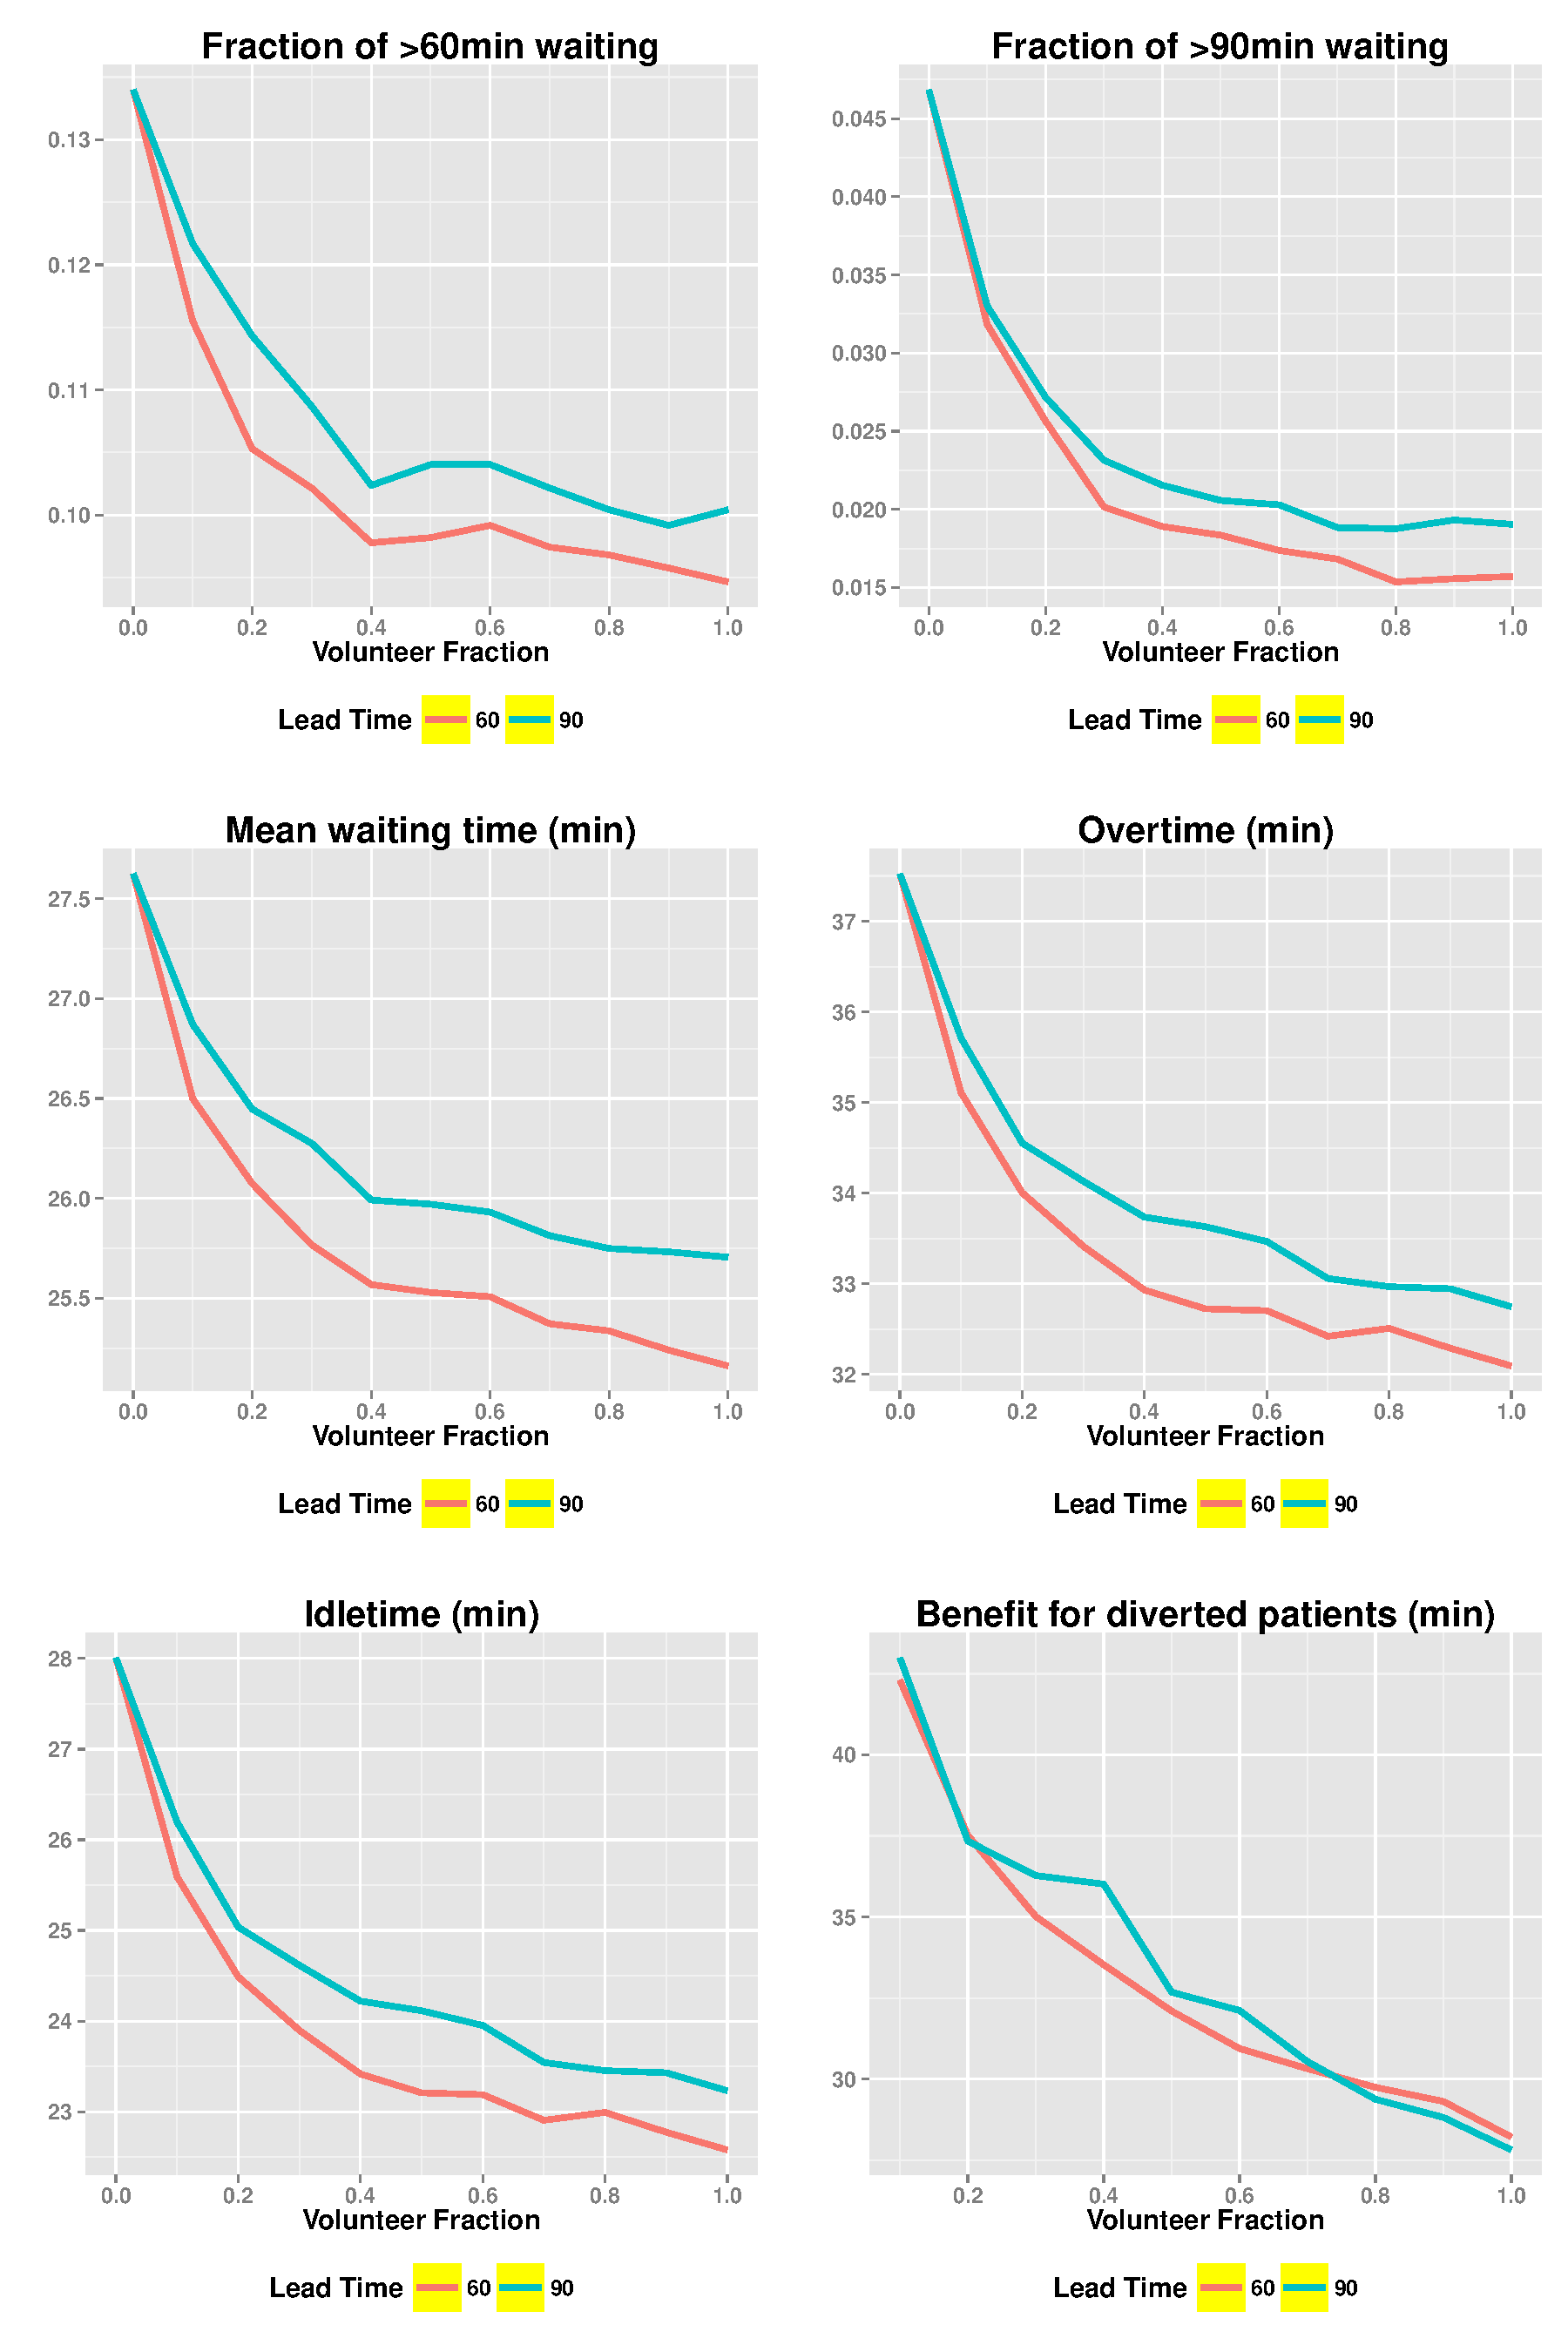
\includegraphics[width=.95\textwidth]{chap3/numeric/pic/3sites_all}
\caption{System performance improvement by diversion.}
\label{fig:3sites_all}
\end{figure}

We also want to note that, as Figure \ref{fig:3sites_all_diversion} shows,
we only diverted very small fraction of patients. Even if all patients
are volunteers, we only diverted less than 3\% of them.
We think this is a desirable property since less changes are easier
to implement. Also since there are only 3 changes per day on average,
the staff can use their domain knowledge to better facilitate those
changes.

\begin{figure}[htp]
\centering
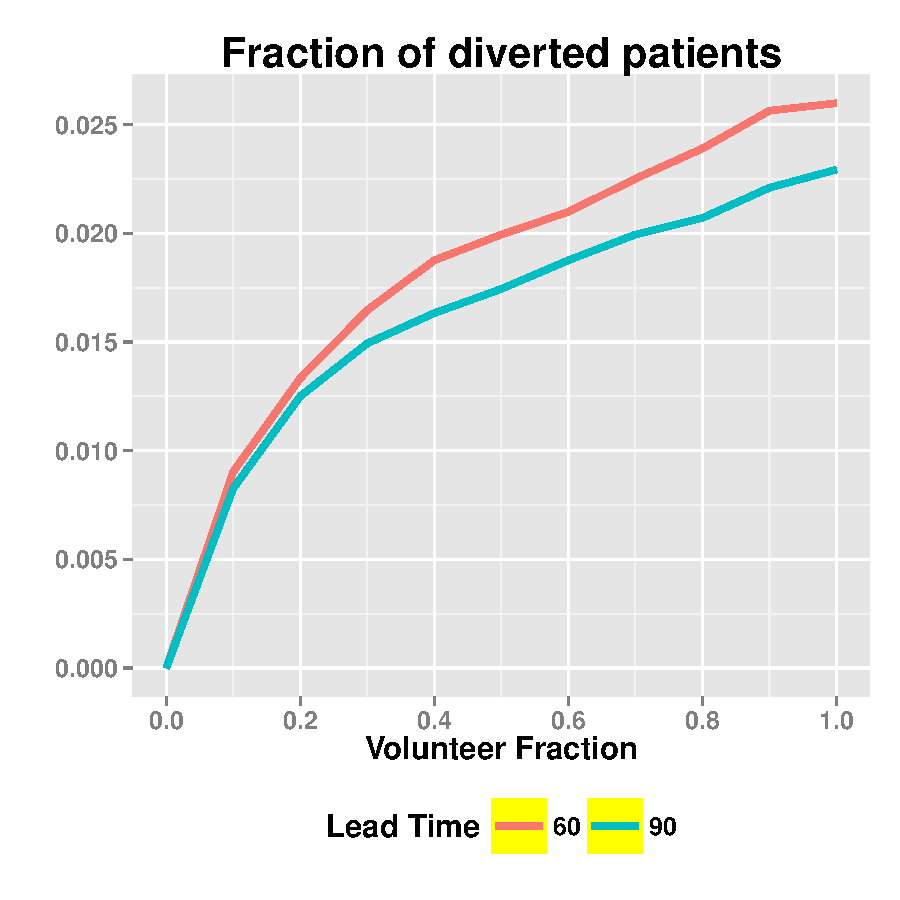
\includegraphics[width=.6\textwidth]{chap3/numeric/pic/3sites_all_diversion}
\caption{Fraction of patients diverted.}
\label{fig:3sites_all_diversion}
\end{figure}

Overall, we think diversions are shown to be a efficient way to
improve system performance for NYP's outpatient MRI sites.
It can significantly improve on patient waiting time, sites overtime
without incurring too many diversions.
